%Note di Ingegneria del Software
%Sommario: MVC MVP MVVM

\cornell{Pattern Model-View}{\begin{itemize}
\item Per supportare diversi utenti con diverse interfacce
\item Evitando duplicazione di codice
\item Senza influenzare le componenti che forniscono funzionalità base
\end{itemize}}

\cornell{MVC}{Model-View-Controller}

\cornell{Model}{È il modello della realtà\\
Contiene la "business logic" del programma.\\
Definisce quindi il modello dei dati e le operazioni che si possono effettuare su questi.\\
Viene progettato tramite tecniche Object-Oriented (Design Pattern)\\
Notifica la View dell'aggiornamento del modello dati (Observer Pattern)}

\cornell{View}{È L'interfaccia utente.\\
Contiene la "presentation logic" del programma\\
Contiene quindi la logica di presentazione.\\
Cattura l'input e delega l'elaborazione al controller.\\
L'aggiornamento può essere fatto secondo: \begin{description}
\item [Push Model] La view deve essere costantemente aggiornata (observer pattern);
\item [Pull Model] La view va a richiedere l'update quanto è opportuno.
\end{description}}

\cornell{Controller}{Contiene la logica di controllo tra model e view, cioè qual'è la reazione agli input dell'utente.\\
Contiene cioè la "application logic"\\
Trasforma quindi le interazioni utente in azioni sui dati.\\
Esiste solitamente un controller per ogni view.\\
Può implementare il strategy pattern (che modifica gli algoritmi che permettono l'interazione utente col model)}

\cornell{UML Classi del Push Model}{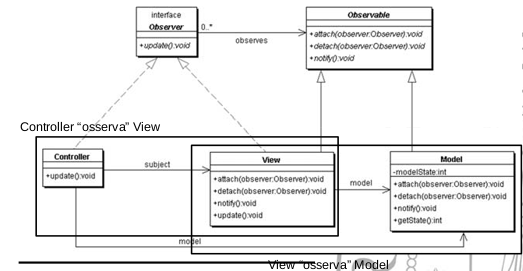
\includegraphics[scale=0.5]{images/61.png}}

\cornell{UML Sequenza del Push Model}{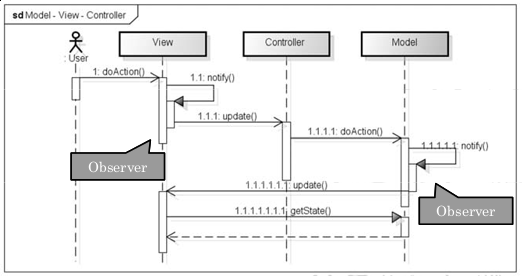
\includegraphics[scale=0.5]{images/62.png}}

\cornell{Conseguenze dell'MVC}{ \begin{itemize}
\item Evita che il team dedicato al front-end vada a modificare la business logic, così come l'inverso
\item Permette parallelismo, separando i "concerns" (Disaccoppiamento)
\item Permette il riuso delle componenti del model
\item Supporto più semplice per nuovi tipi di client (Basta creare nuovi view e controller)
\item Miglior Manutenzione e Testing
\item Maggiore Complessità di progettazione (Ci saranno più classi, per garantire la separazione, ma tali classi avranno minori responsabilità)
\end{itemize}}

\cornell{MVP}{Model-View-Presenter\\
Usato soprattutto su Android}

\cornell{View}{Stiamo spostando responsabilità via dalla view, rendendola "stupida", privandola della presentation logic. Così diventa solo un template di visualizzazione (in Android è un file XML)}

\cornell{Presenter}{Il presenter, tramite dei getter e dei setter, aggiorna e osserva la vista (fungendo da man-in-the-middle)}

\cornell{Conseguenze dell'MVP}{Il presenter è facilmente testabile, facendo semplicemente un Mock della View}

\cornell{UML Dell'MVP}{ 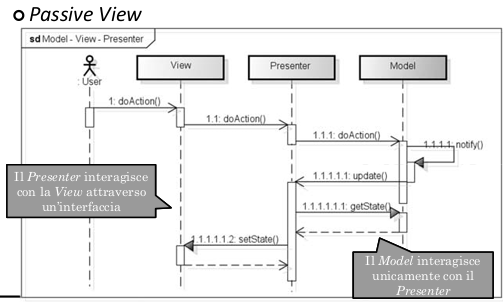
\includegraphics[scale=0.5]{images/63.png}}

\cornell{MVVM}{Model-View-ViewModel\\
Separa lo sviluppo della UI da quello della business Logic.\\
La ViewModel è una proiezione del modello creata per una vista, nel modello resta solamente la validazione.\\
Viene eseguito un binding con la vista ed il modello tramite la ViewModel così che dati ed operazioni possano essere eseguiti su una UI.\\
La view Diventa dichiarativa (usando linguaggi di markup).\\
Avviene un 2-way data binding con proprietà del ViewModel e la view non possiede più lo stato dell'applicazione.\\
Tra View e ViewModel vi è un doppio observer pattern.\\
MVVM viene usato da AngularJS.}

\cornell{Schema Esplicativo}{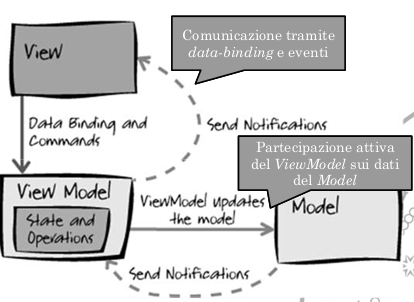
\includegraphics[scale=0.5]{images/64.png}}

% vi: spell spelllang=it,en
